\section{Drawing Mechanism}

The drawing system is comprised by a pool of numbers (balls) that will be randomly chosen for every transaction (ticket) without replacement. We can calculate the chances for $M$ divisions (number of balls in a single ticket for a single transaction) via the hypergeometric distribution as follows \cite{feller}:

\begin{equation}
    p_m = \frac{\binom{M}{m}\binom{N-M}{M-m}}{\binom{N}{M}} = \frac{(M!)^2((N-M)!)^2}{m!N!((M-m)!)^2(m-2M+N)!}
\end{equation}

where $m$ is the number of matching balls for a winning ticket and $N$ is the total number of balls in the pool. To ensure that the largest dividend is paid out at least four times annually, $N$ must satisfy the following condition:

\begin{equation} \label{ncond}
    p_M \geq \frac{4}{ATX} \Leftrightarrow N! < \frac{1}{4} ATX \cdot M! (N-M)!
\end{equation}

A solution to (\ref{ncond}) can be found numerically and may be computed off-chain by finding the largest possible value iteratively or via binary search.

Finally, we can evaluate the TRF in its complete form:

\begin{equation} \label{trff}
    w_m = \frac{1}{M} \Bigg[c_0 + \frac{(K-c_0)t}{t+r}\Bigg] \Bigg(\frac{\binom{M}{m}\binom{N-M}{M-m}}{\binom{N}{M}}\Bigg)^{-1} 
    \begin{dcases}
    \frac{\Xi}{ATX} & \mu \leq g \\
    g & \mu > g
    \end{dcases}
\end{equation}

(\ref{trff}) will be calculated for every single transaction. The value of $M$ may be chosen through governance decisions.

An example table for the payout and probability vectors can be seen below ($\Xi = \$50,000,000$, $ATX = 31,536,000$, $g = \$3$, $M=6$, $c = 1$).

\vspace{1em}
\begingroup
            \centering
            \begin{tabular}{||c | c ||}
            \hline
            $p_m \: [\%]$ & $w_m \: [\$]$ \\[0.5ex]
            \hline
            42.66 & 0.62  \\
            15.69 & 1.69 \\
            2.39 & 11.06 \\
            0.15 & 176.89 \\
            3.23e-3 & 8181.33 \\
            
            1.41e-5 & 1,865,342.25 \\
            \hline
            \end{tabular}
            \par
\endgroup
\vspace{1em}
            

We can see that for $\mu \leq g$

\begin{equation}
    \langle p,w\rangle ATX = \sum_{m=1}^M w_m p_m\cdot ATX = \Xi
\end{equation}

For protocols with smaller fees where $\mu>g$ we explore graph classification models and other strategies in order for them to remain competitive.
We discuss higher expected outcomes through the probability vector $p_m$ by increasing the number of tickets for a single transaction in the aforementioned follow up paper.

\clearpage

To gain a better understanding of how the Transfer Reward Function works together with the Optimistic Solution, we have plotted the isolines for increasing transaction fees in \autoref{fig:fig} on different logarithmic scales. We can see that as the transaction fee increases, the curve of the TRF initally shifts upwards and the rewards for the different tiers increase with it. We can observe that the curve converges towards the equilibrium state of $g \geq \Xi/ATX$. At that point the TRF stops shifting upwards and consequently the magnitude of rewards are dependent on the size of the pool, the total number of fluid transactions and independent of the transaction fee paid by the user. The fee paid by the user thus only affects the payouts when they are low enough, and it doesn't affect the chances of receiving a reward. The same holds true for the ESC and other mechanisms aimed at increasing the expected value for a fluid transaction.


\begin{figure}
\begin{subfigure}{.5\textwidth}
  \centering
  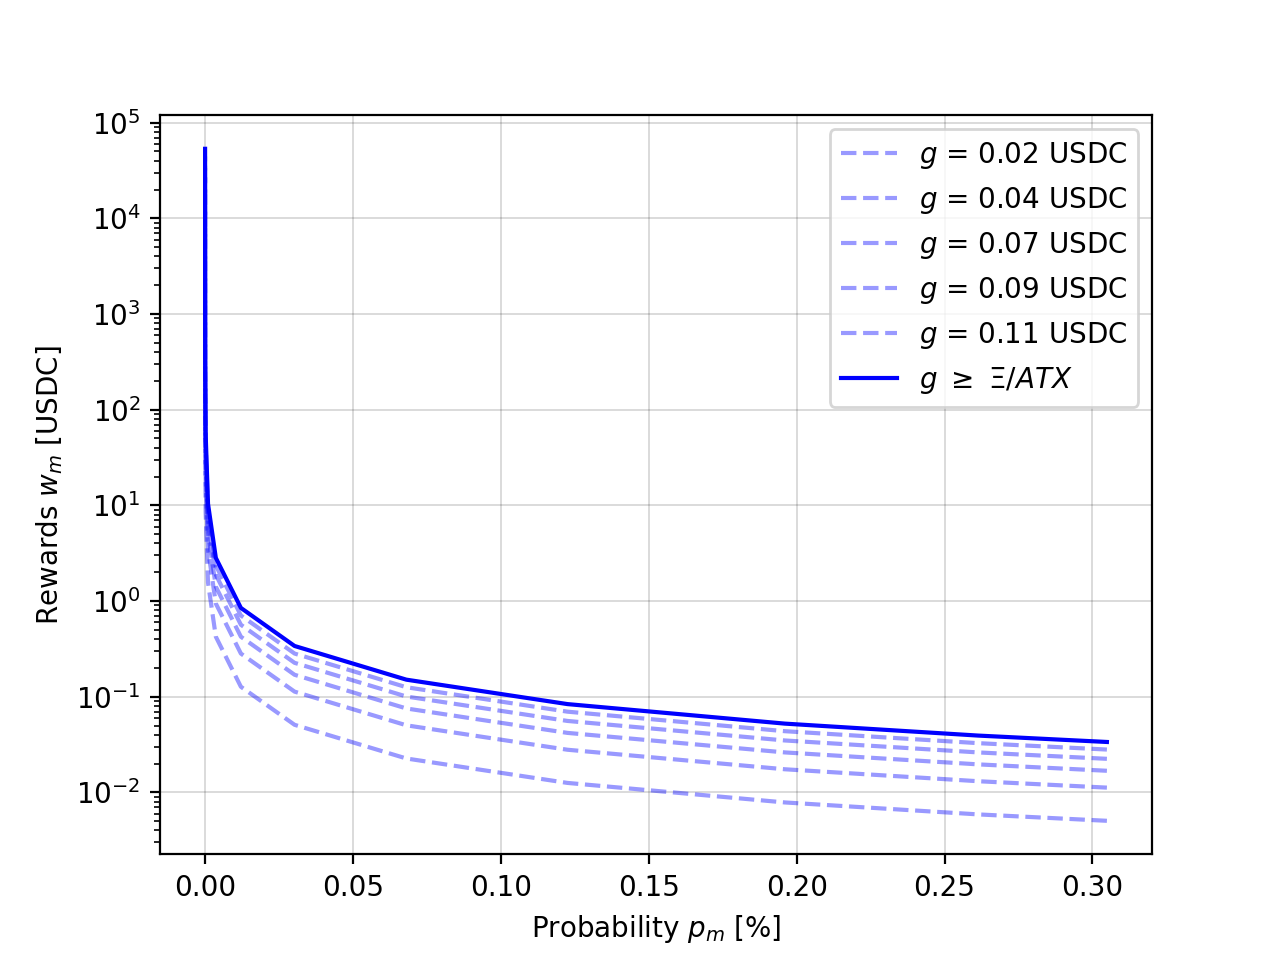
\includegraphics[width=1.1\linewidth]{images/trf4.png}
  \caption{y-log scale}
  \label{fig:sfig1}
\end{subfigure}%
\begin{subfigure}{.5\textwidth}
  \centering
  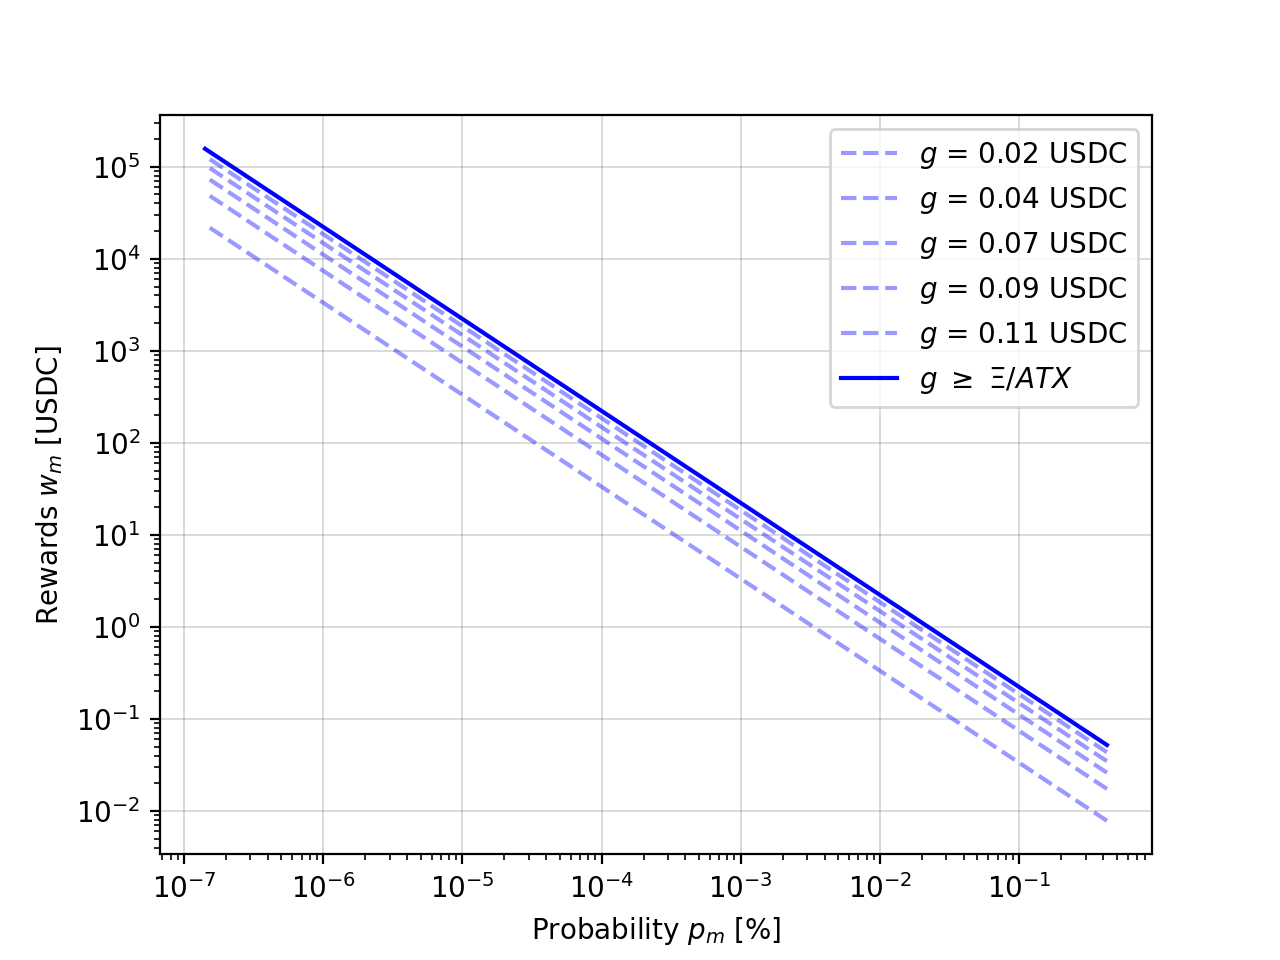
\includegraphics[width=1.1\linewidth]{images/trf3.png}
  \caption{log-log scale}
  \label{fig:sfig2}
\end{subfigure}
\caption{Plots of the TRF with the Optimistic Solution}
\label{fig:fig}
\end{figure}

\clearpage